%!TEX TS-program = xelatex  
%!TEX encoding = UTF-8 Unicode  
      
\documentclass[a4paper, 11pt]{article}
\usepackage[top=1.5in, bottom=1.5in, left=1.0in, right=1.0in]{geometry} 
\usepackage{indentfirst}        
\usepackage{float}
\usepackage{amsmath}
\usepackage{hyperref}
\usepackage{graphicx}


\title{ARMA-GARCH}
\author{SHIHENG SHEN}
\date{\today}
\begin{document}
\maketitle

\section{Data}
\subsection{Data Source}
HadCRUT4 is a gridded dataset of global historical surface temperature anomalies relative to a 1961-1990 reference period. Data are available for each month since January 1850, on a 5 degree grid. The dataset is a collaborative product of the Met Office Hadley Centre and the Climatic Research Unit at the University of East Anglia. \\ $url = $\url{http://www.metoffice.gov.uk/hadobs/hadcrut4/data/current/time_series/HadCRUT.4.5.0.0.monthly_ns_avg.txt}.
\subsection{Brief Data Description}
The gridded data are a blend of the CRUTEM4 land-surface air temperature dataset and the HadSST3 sea-surface temperature (SST) dataset. The dataset is presented as an ensemble of 100 dataset realisations that sample the distribution of uncertainty in the global temperature record given current understanding of non-climatic factors affecting near-surface temperature observations. This ensemble approach allows characterisation of spatially and temporally correlated uncertainty structure in the gridded data, for example arising from uncertainties in methods used to account for changes in SST measurement practices, homogenisation of land station records and the potential impacts of urbanisation.
The HadCRUT4 data are neither interpolated nor variance adjusted.\par
Below is a graph provided by \url{www.metoffice.gov.uk}:
\begin{figure}[H]
\centering
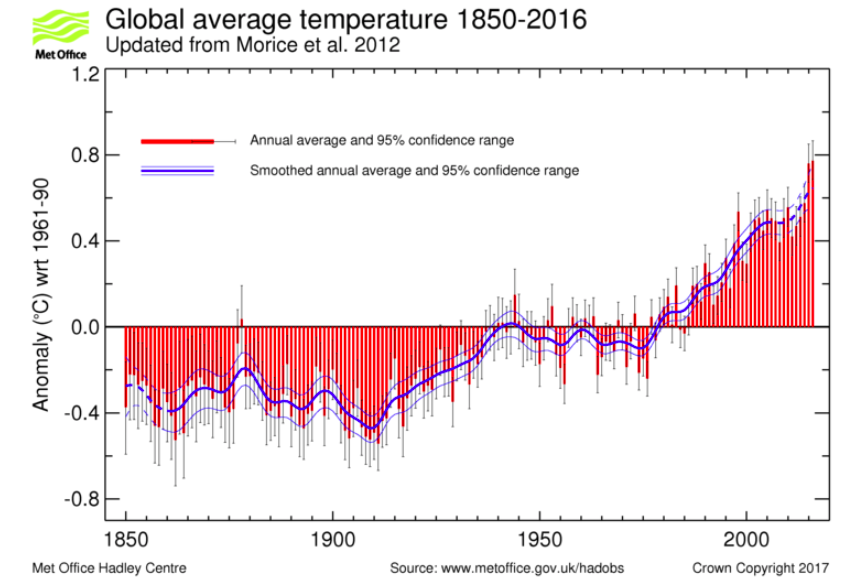
\includegraphics[scale=.30]{global.png}
\end{figure} 

\subsection{Loading the Data into R}
For our purpose, we are not interested in the spatial distribution, so we only use the \textit{Global Mean}.\\
Loading the data into R:
\begin{verbatim}
library(curl)
tmpf <- tempfile()
curl_download(url, tmpf)
gtemp <- read.table(tmpf)[, 1:2]
temp = gtemp$V2[1:2004]
\end{verbatim}
\indent We only use the first two columns: \textit{time and monthly global mean}. We pick the first 2004 observations, which is monthly data from $1850 \sim 2016$, so that the data has complete periods.\par
The time series of $temp$ is shown below:
\begin{figure}[H]
\centering
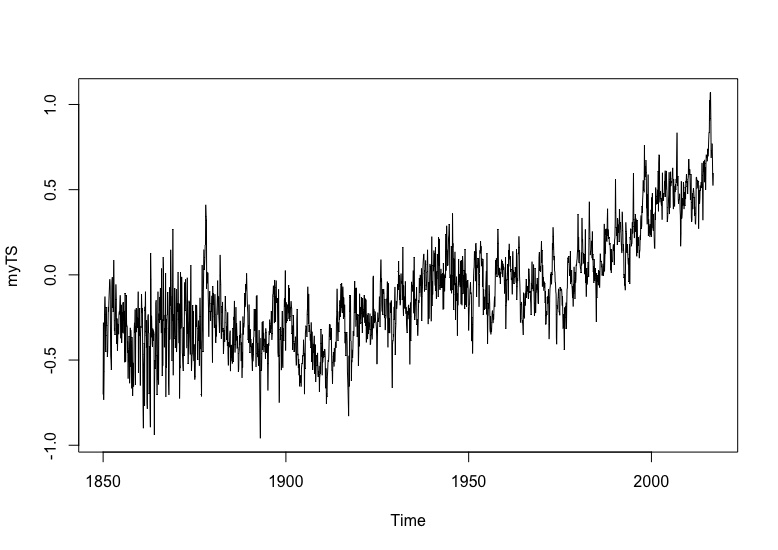
\includegraphics[scale=.45]{temp.png}
\end{figure}

\section{Dealing with the time series}

\subsection{Decompose}
The first thing we might want to do is to wipe out the seasonal component and the time trend. There're many approaches to do it in R. We choose to use the $decompose() provided by \{stats\}$. Looking at the time series, we think a additive model should be appropriate. Therefore, decompose the time series using the following code:

\begin{verbatim}
library(TSA)
myTS = decompose(ts(as.numeric(temp), frequency = 12))
# TS$x = TS$seasonal + TS$trend + TS$random(residuals) 
res = myTS$random
# wipe out NAs
res.noNA = res[7:2004] 
res = res.noNA[1:1992]
\end{verbatim}
\indent The $res$ now is free of seasonal component and time trend. The following graph illustrate the components.
\begin{figure}[H]
\centering
\caption{original ts, time trend, additive seasonal component, residuals}
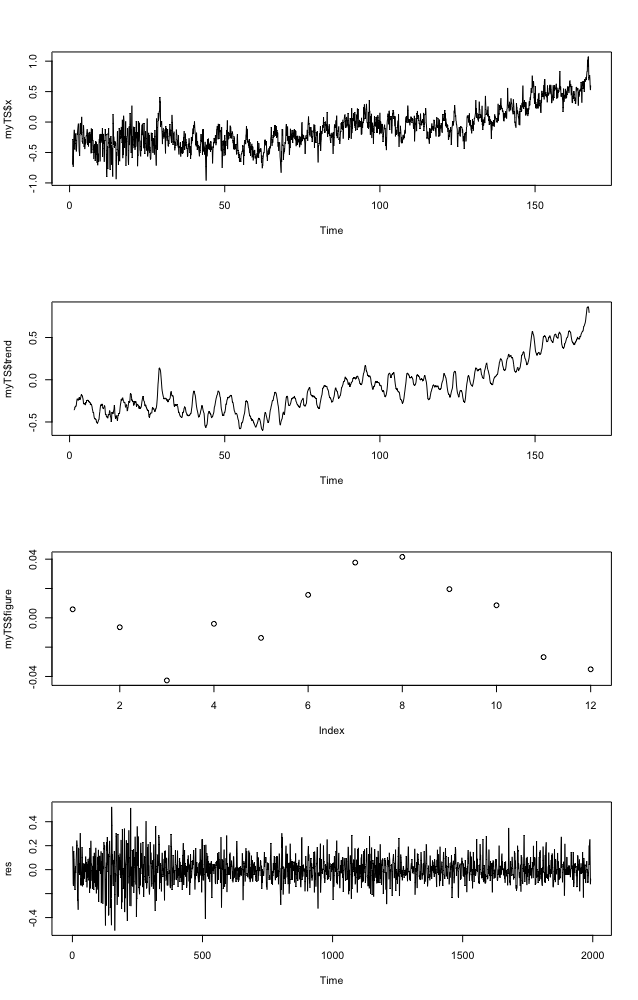
\includegraphics[scale=.60]{component.png}
\end{figure}

\indent brief results:
\begin{verbatim}
> mean(res)
[1] 0.0002073084
> var(res)
[1] 0.01139539
> adf.test(res)

	Augmented Dickey-Fuller Test

data:  res
Dickey-Fuller = -18.364, Lag order = 12, p-value = 0.01
alternative hypothesis: stationary
\end{verbatim}
\indent So we can convince ourself that the time series $res$ is stationary.

\subsection{Build a \textit{ARMA(p, q)} for \textit{res}}
For simplicity, we use $auto.arima()$ from $\{forecast\}$.
\begin{verbatim}
library(forecast)
armamodel = auto.arima(res)
\end{verbatim}
\indent The results are all significant:

\begin{verbatim}
> armaModel
Series: res 
ARIMA(1,0,2) with zero mean     

Coefficients:
          ar1     ma1     ma2
      -0.5179  0.7198  0.1597
s.e.   0.1572  0.1550  0.0326

sigma^2 estimated as 0.01096:  log likelihood=1670.58
AIC=-3333.17   AICc=-3333.15   BIC=-3310.78
> Box.test(arma_residual, type = 'Ljung-Box')

	Box-Ljung test

data:  arma_residual
X-squared = 0.086116, df = 1, p-value = 0.7692
\end{verbatim}

\indent The $ARMA(1, 2)$ success in making the arma residual independent. 



\subsection{GARCH}
One can be pretty satisfied with the results right now. Yet Looking at the plot of arma residual:
\begin{figure}[H]
\centering
\caption{arma residual}
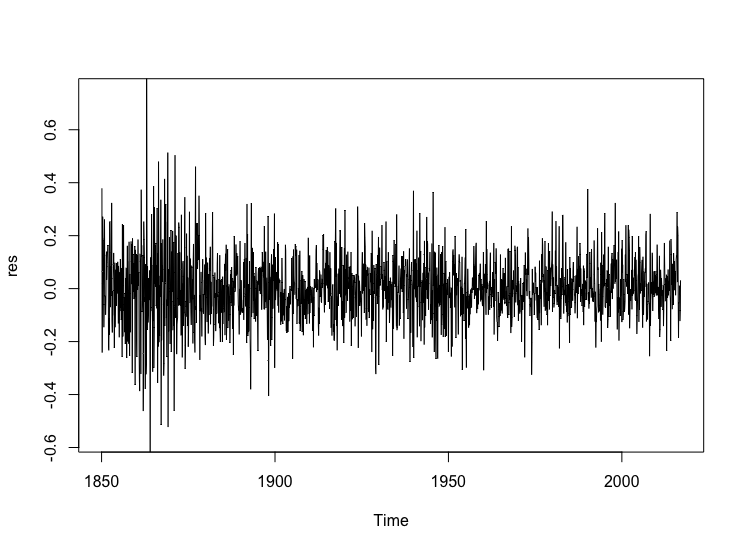
\includegraphics[scale=.60]{armares.png}
\end{figure}

\indent It makes us wondering if it has $ARCH$ effect. Using $arch.test$ from $\{aTSA\}$ to perform the $LM-Test$:
\begin{verbatim}
library(aTSA)
> my.arma = arima(res, order = c(1, 0, 2))
> arch.test(my.arma)
ARCH heteroscedasticity test for residuals 
alternative: heteroscedastic 

Portmanteau-Q test: 
     order   PQ p.value
[1,]     4  188       0
[2,]     8  233       0
[3,]    12  546       0
[4,]    16  665       0
[5,]    20  727       0
[6,]    24 1035       0
Lagrange-Multiplier test: 
     order   LM  p.value
[1,]     4 1188 0.00e+00
[2,]     8  577 0.00e+00
[3,]    12  341 0.00e+00
[4,]    16  199 0.00e+00
[5,]    20  155 0.00e+00
[6,]    24  127 2.22e-16
\end{verbatim}
\indent It supports our doubt. Therefore we have the motive to build a $GARCH$ model. We decide to use the package $rugarch$.\par
Though we do know that using $GARCH$ may change the order of $ARMA$, yet given our significance of $ARMA$ model and the difficulty in determing the order, we decide to only model the variance in 'sGARCH'(standard GARCH model):
\begin{equation*}
	\sigma_t^2 = (w + \sum_{j = 1}^m \zeta_j v_{jt}) + \sum_{j = 1}^q \alpha_j \varepsilon_{t-j}^2 + \sum_{j = 1}^p \beta_j \sigma_{t-j}^2
\end{equation*} 
\indent So we wrote a function:
\begin{verbatim}
library(rugarch)
my_sGARCH_test <- function(p, q, m, n, ts.data = res)
{
	# I use include.mean = FALSE after trying TRUE
	# to find out insignificance
    myspec=ugarchspec(variance.model = list(model = "sGARCH", garchOrder = c(p, q)), 
    	mean.model = list(armaOrder = c(m, n), include.mean = FALSE), 
    	distribution.model = "norm")
    myfit=ugarchfit(myspec,data=ts.data, solver="solnp")
    return(myfit)  
}
\end{verbatim}
\indent After trying a few times from $(1, 0)$ to $(5, 5)$, \textit{GARCH(1 ,1)} is the most satisfying model.
\begin{verbatim}
> fit
> fit = my_sGARCH_test(1, 1, 1, 2, res)
> fit

*---------------------------------*
*          GARCH Model Fit        *
*---------------------------------*

Conditional Variance Dynamics 	
-----------------------------------
GARCH Model	: sGARCH(1,1)
Mean Model	: ARFIMA(1,0,2)
Distribution	: norm 

Optimal Parameters
------------------------------------
        Estimate  Std. Error     t value Pr(>|t|)
mu      0.000021    0.000031  6.6898e-01 0.503509
ar1     0.656721    0.017318  3.7921e+01 0.000000
ma1    -0.829580    0.000010 -7.9768e+04 0.000000
ma2    -0.165154    0.000037 -4.4098e+03 0.000000
omega   0.000063    0.000020  3.2269e+00 0.001251
alpha1  0.025901    0.003165  8.1827e+00 0.000000
beta1   0.966408    0.002955  3.2699e+02 0.000000

Robust Standard Errors:
        Estimate  Std. Error     t value Pr(>|t|)
mu      0.000021    0.000026  7.9059e-01 0.429185
ar1     0.656721    0.017500  3.7527e+01 0.000000
ma1    -0.829580    0.000004 -2.2586e+05 0.000000
ma2    -0.165154    0.000068 -2.4225e+03 0.000000
omega   0.000063    0.000020  3.1854e+00 0.001446
alpha1  0.025901    0.003232  8.0135e+00 0.000000
beta1   0.966408    0.001365  7.0795e+02 0.000000

LogLikelihood : 1960.533 

Information Criteria
------------------------------------
                    
Akaike       -1.9614
Bayes        -1.9417
Shibata      -1.9614
Hannan-Quinn -1.9542

Weighted Ljung-Box Test on Standardized Residuals
------------------------------------
                         statistic p-value
Lag[1]                      0.4938  0.4823
Lag[2*(p+q)+(p+q)-1][8]    53.1672  0.0000
Lag[4*(p+q)+(p+q)-1][14]   71.9866  0.0000
d.o.f=3
H0 : No serial correlation

Weighted Ljung-Box Test on Standardized Squared Residuals
------------------------------------
                        statistic   p-value
Lag[1]                      12.76 3.533e-04
Lag[2*(p+q)+(p+q)-1][5]     17.44 9.751e-05
Lag[4*(p+q)+(p+q)-1][9]     25.41 7.594e-06
d.o.f=2

Weighted ARCH LM Tests
------------------------------------
            Statistic Shape Scale  P-Value
ARCH Lag[3]   0.01376 0.500 2.000 0.906619
ARCH Lag[5]   3.57130 1.440 1.667 0.216963
ARCH Lag[7]  11.37620 2.315 1.543 0.008741

Nyblom stability test
------------------------------------
Joint Statistic:  2.3108
Individual Statistics:              
mu     0.09865
ar1    0.33227
ma1    0.47659
ma2    0.51154
omega  0.12277
alpha1 0.44943
beta1  0.24423

Asymptotic Critical Values (10% 5% 1%)
Joint Statistic:     	 1.69 1.9 2.35
Individual Statistic:	 0.35 0.47 0.75

Sign Bias Test
------------------------------------
                   t-value      prob sig
Sign Bias            1.811 0.0702699   *
Negative Sign Bias   2.571 0.0102247  **
Positive Sign Bias   3.036 0.0024298 ***
Joint Effect        21.325 0.0000901 ***


Adjusted Pearson Goodness-of-Fit Test:
------------------------------------
  group statistic p-value(g-1)
1    20     57.60    9.222e-06
2    30     68.57    4.742e-05
3    40     87.64    1.333e-05
4    50    104.89    6.078e-06


Elapsed time : 0.3056059
\end{verbatim}

\indent Substract the standardized(w.r.t. the variance model) residuals $z$, which is $z = \cfrac{residuals(fit)}{sigma(fit)}$.

\begin{verbatim}
z = residuals(fit) / sigma(fit)
plot.ts(z)
\end{verbatim}

\begin{figure}[H]
\centering
\caption{z}
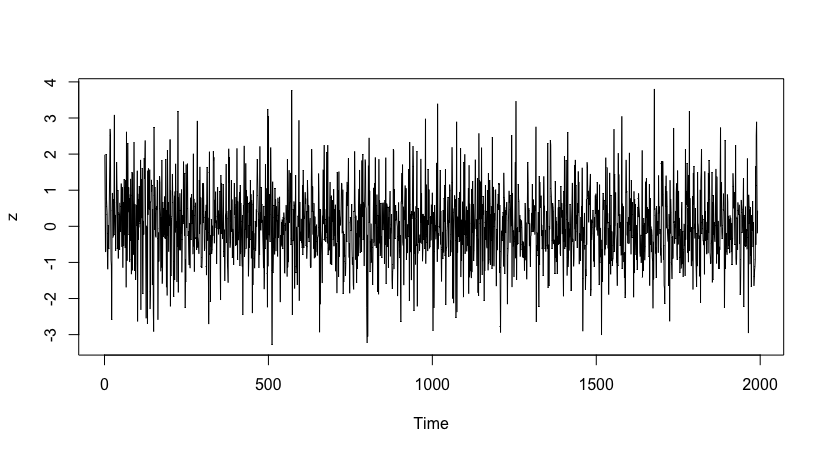
\includegraphics[scale=.40]{z.png}
\end{figure}

\indent We can compute the mean and variance of $z$:
\begin{verbatim}
> mean(z)
[1] 0.02010495
> var(z)
[1] 1.00525
\end{verbatim} 
\indent And then, just for fun, plot a normal sample series with the same parameters:
\begin{verbatim}
plot.ts(rnorm(1992, 0.2010495, 1.00525))
\end{verbatim}

\begin{figure}[H]
\centering
\caption{simulation of using rnorm}
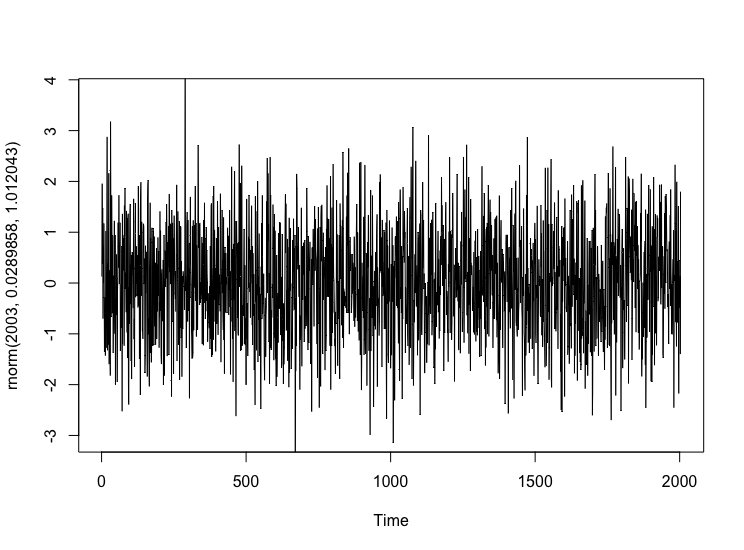
\includegraphics[scale=.40]{rnorm.png}
\end{figure}

\indent At least a human can't distinguish between them anymore. But what we most care about is whether standardized squared residuals can pass the $LM-Test$(substracting from the above long result):

\begin{verbatim}
Weighted ARCH LM Tests
------------------------------------
            Statistic Shape Scale  P-Value
ARCH Lag[3]   0.01376 0.500 2.000 0.906619
ARCH Lag[5]   3.57130 1.440 1.667 0.216963
ARCH Lag[7]  11.37620 2.315 1.543 0.008741
\end{verbatim}

We can see our model successfully wipes out ARCH effect at smaller lags, but fails at $lag[7]$. This is the best `sGARCH' can give with respest to our data.


\textbf{Graphical Diagnostics:}\par
\text{rugarch} provide a function to plot a "uGARCHfit" obeject.\par
ex. density smmothed to normal distribution:
\begin{figure}[H]
\centering
\caption{Empirical Density of Standardized Residuals}
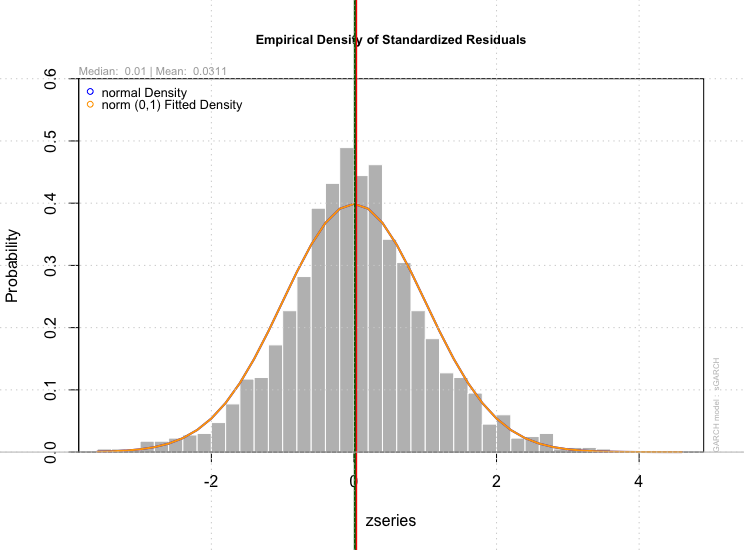
\includegraphics[scale=.60]{density.png}
\end{figure}
 
qqplot:
\begin{figure}[H]
\centering
\caption{qqplot of $z$}
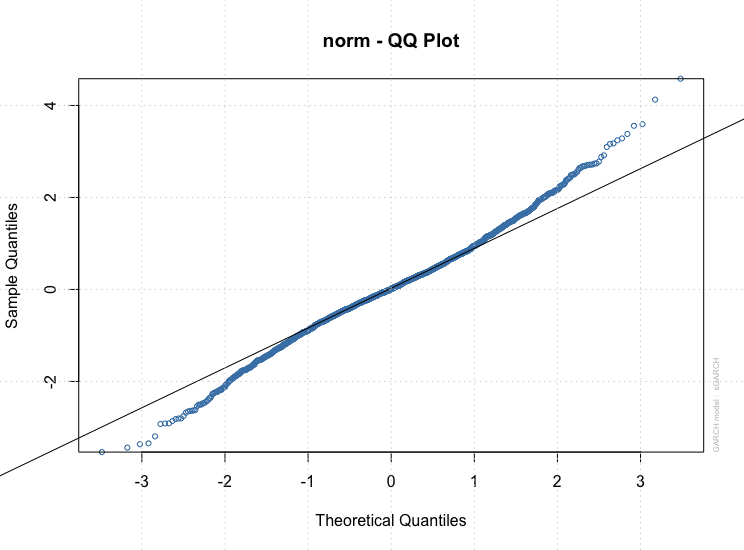
\includegraphics[scale=.60]{qqplot.png}
\end{figure}

\indent We can see that $z$ is skewed, which might be correlated with long lags' heterodasticity.\par

\textbf{Conclusion}: 'sGARCH' have improved the model in the intuitive sense and to some extent fix the heterodasticity. 




\end{document}